\chapter{Divide-et-impera}\label{chap:divide-et-impera}
\section{Introduzione}
Giunti a questo punto della trattazione, è arrivato il momento di parlare delle
tecniche per la risoluzione di problemi, ovvero di quelle tecniche che permettono
di arrivare alla definizione di un algoritmo per la risoluzione di un particolare
problema.

Esiste un'ampia di gamma di categorie di problemi, tra le quali troviamo:
\begin{itemize}
    \item \emph{Problemi decisionali}: l'obiettivo è riuscire a stabilire se il
    dato in ingresso soddisfa o meno una proprietà;
    \item \emph{Problemi di ricerca}: l'obiettivo è ricercare all'interno
    dell'insieme dei dati di input un sottoinsieme di dati che soddisfano una
    certa proprietà;
    \item \emph{Problemi di ottimizzazione}: in un insieme di soluzioni alle
    quali è associata una funzione di costo, l'obiettivo è trovare la soluzione
    di costo minimo;
\end{itemize}
Le tecniche per la ricerca di soluzioni sono molteplici e nel corso della
trattazione ne approfondiremo diverse. In questo capitolo, iniziamo a vedere
la tecnica del \emph{Divide-et-impera}.

\begin{definition}[Tecnica del Divide-et-impera]
    La tecnica del Divide-et-impera prevede che il problema da risolvere venga
    suddiviso in sotto-problemi indipendenti e che le soluzioni ai sotto-problemi
    vengano combinate per ottenere la soluzione al problema di partenza.
\end{definition}\noindent
La definizione lascia intendere molto chiaramente la simbiosi che esiste tra
algoritmi \emph{Divide-et-impera} e ricorsione. Infatti, la suddivisione in
sotto-problemi viene realizzata applicando ricorsivamente l'algoritmo ad un
sottoinsieme dei dati di input.

\bigskip\noindent
L'approccio \emph{Divide-et-impera} si compone di tre fasi:
\begin{itemize}
    \item \emph{Divide}: il problema viene suddiviso in sotto-problemi indipendenti;
    \item \emph{Impera}: vengono risolti i sotto-problemi;
    \item \emph{Combina}: le soluzioni dei sotto-problemi vengono combinate per
    ottenere la soluzione al problema di partenza;
\end{itemize}
\begin{note}
    La tecnica del \emph{Divide-et-impera} trova applicazione soprattutto negli
    ambiti dei \emph{problemi decisionali} e \emph{di ricerca}.
\end{note}\noindent
Vediamo un esempio tipico di applicazione della tecnica
\emph{Divide-et-impera}.
\begin{problem}[Problema della Torre di Hanoi]
    Quello della Torre di Hanoi è un problema matematico molto famoso. Esistono
    tre pioli e $n$ dischi di dimensione diversa. Inizialmente i dischi sono
    impilati in ordine decrescente sul piolo di sinistra. Lo scopo del gioco è
    riuscire a impilare quegli stessi dischi in ordine decrescente sul piolo di
    destra.
    
    Ad ogni mossa è possibile spostare un disco ed è possibile usare il piolo
    centrale come appoggio. L'importante è non posizionare mai un
    disco sopra uno più piccolo.

    \bigskip
\begin{minicode}{Implementazione algoritmo per risoluzione della Torre di Hanoi}
\ind hanoi(\bc{int} n, \bc{int} src, \bc{int} dest, \bc{int} aux)\\
    \indf if (n == 1) then\\
        print src $\to$ dest\\
    \indf else\\
        hanoi(n-1, src, aux, dest)\hfill\com{Sposta $n-1$ dischi sul piolo ausiliario}
        print src $\to$ dest\hfill\com{Sposta il disco più grande}
        hanoi(n-1, aux, src, dest)\hfill\com{Sposta $n-1$ dischi sul piolo finale}
\end{minicode}\noindent
    In questo codice è evidente la suddivisione in sotto-problemi in quanto
    l'invocazione \texttt{hanoi(n-1, src, aux, dest)} sposta tutti i dischi tranne
    l'ultimo sul piolo ausiliario usando il piolo che sarebbe di destinazione come
    piolo d'appoggio. Quindi, sposta il disco rimasto, il più grande, sul piolo
    di destinazione. L'invocazione \texttt{hanoi(n-1, aux, dest, src)}
    sposta di nuovo gli $n-1$ dischi di prima sul piolo di destinazione.

    \bigskip\noindent È interessante provare a studiare la complessità di questa
    soluzione. La funzione di ricorrenza è la seguente:
    \[T(n)=2T(n-1)+1\]
    e per il \hyperref[def:21]{Teorema delle ricorrenze lineari di ordine costante}
    il costo di questo algoritmo è $\Theta(2^n)$, che nonostante sia un costo
    esponenziale è comunque il migliore possibile in quanto è dimostrabile
    l'ottimalità della soluzione proposta.
\end{problem}

\paragraph{Convenienza degli algoritmi Divide-et-impera}
L'utilizzo di una qualsiasi tecnica per la risoluzione di problemi non sempre
permette di arrivare ad una soluzione ottima o anche solo conveniente.
Ad esempio, la seguente implementazione ricorsiva della funzione di ricerca del
minimo non è migliore della sua controparte iterativa:
\begin{minicode}{Implementazione minrec per la ricerca ricorsiva del minimo}
    \ind\bc{int} minrec(\bc{int}[] A, \bc{int} i, \bc{int} j)\\
        \indf if (i == j) then\\
            return A[i]\\
        \indf else\\
            m = $\lfloor$(i + j) / 2$\rfloor$\\
            return min(minrec(A, i, m), minrec(A, m + 1, j))
\end{minicode}\noindent
La \emph{funzione di ricorrenza} di questa soluzione è:
\[T(n)=\begin{cases}
    2T(n/2)+1 & n>1\\
    1 & n\leq1
\end{cases}\]
e per il \emph{\hyperref[def:19]{Teorema delle ricorrenze lineari con
partizione bilanciata - Rid}} vale $T(n)=\Theta(n)$ che è la stessa
\emph{complessità} della versione iterativa dell'algoritmo. Di conseguenza,
in questo caso non conviene usare la tecnica del \emph{Divide-et-impera} perché
l'algoritmo ottenuto è più complicato di quello che già conoscevamo.

\section{Algoritmo Quicksort}
All'inizio della trattazione abbiamo già esaminato un algoritmo di ordinamento
basato sul \emph{Divide-et-impera}: l'algoritmo \emph{merge sort}.

\subsection{Principi di funzionamento}
Il \emph{Quicksort} è un altro algoritmo di ordinamento, basato anch'esso su
\emph{Divide-et-impera}, che riceve in input un vettore $A[1\dots n]$ e due indici $lo$ e
$hi$ tali che $1\leq lo\leq hi\leq n$.

Nella fase di \emph{divide} viene scelto un valore $p\in A[lo\dots hi]$ detto
\emph{perno} o \emph{pivot}. Quindi, tutti gli elementi del vettore vengono
permutati in modo da portare tutti i valori più piccoli del \emph{pivot} alla sua
sinistra e gli altri alla sua destra.

\begin{figure}[h!]
    \centering
    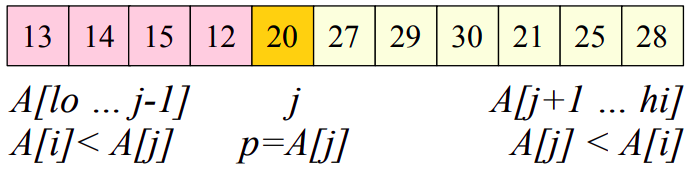
\includegraphics[width=0.7\textwidth]{quicksort1.png}
    \caption{Posizionamento dei valori dopo la scelta del \emph{pivot}}
\end{figure}\noindent
Nella fase di \emph{Impera} vengono ordinati i due sottoarray $A[lo\dots j-1]$
e $A[j+1\dots hi]$ e infine nella fare di \emph{Combina} non serve fare nulla in
quanto il vettore risulta già ordinato.

\begin{figure}[h!]
    \centering
    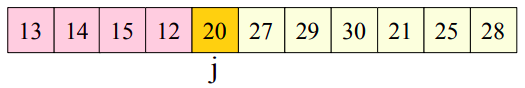
\includegraphics[width=0.7\textwidth]{quicksort2.png}
    \caption{Vettore ordinato al termine della fase di \emph{Impera}}
\end{figure}

\newpage
\subsection{Implementazione}
\begin{minicode}{Implementazione dell'algoritmo Quicksort}
    \ind quicksort(\bc{ITEM}[] A, \bc{int} lo, \bc{int} hi)\\
        \indf if (lo < hi) then\\
            \bc{int} j = pivot(A, lo, hi)\hfill\com{Calcola il \emph{pivot}}
            quicksort(A, lo, j - 1)\hfill\com{Ordina il sottoarray sinistro}
            quicksort(A, j + 1, hi)\hfill\com{Ordina il sottoarray destro}

    \com{Funzione per la ricerca del \emph{pivot}}
    \rmbreak\ind\bc{int} pivot(\bc{ITEM}[] A, \bc{int} lo, \bc{int} hi)\\
        \bc{ITEM} pivot = A[lo]\hfill\com{Scelta del valore del \emph{pivot}}
        \bc{int} j = lo\hfill\com{Indice del \emph{pivot}}
        \indf for (i = lo + 1 to hi) do\\
            \indff if (A[i] < pivot) then\\
                j = j + 1\hfill\com{Aggiorna l'indice del \emph{pivot}}
                swap(A, i, j)\hfill\com{Scambia di posizione gli elementi agli indici $i$ e $j$}
        \indf A[lo] = A[j]\\
        \indf A[j] = pivot\hfill\com{Mette in posizione $j$ il \emph{pivot}}
        \indf return j\\

    \com{Funzione ausiliaria per lo scambio di posizione di due elementi}
    \rmbreak\ind swap(\bc{ITEM}[] A, \bc{int} i, \bc{int} j)\\
        \bc{int} tmp = A[i]\\
        A[i] = A[j]\\
        A[j] = tmp
\end{minicode}

\subsection{Costo computazionale}
Per studiare il costo della funzione principale \texttt{quicksort} analizziamo
le funzioni ausiliarie. La \texttt{swap} è banale e ha un costo
$\Theta(1)$, mentre la \texttt{pivot} costa $\Theta(n)$ perché va a confrontare
il \emph{pivot} con ogni elemento dell'array. Per il costo della
\texttt{quicksort} consideriamo separatamente il caso pessimo il caso migliore.

\bigskip\noindent
Il caso pessimo è quello in cui la scelta del \emph{pivot} porta sempre ad avere
due sottoarray di dimensione $0$ e $n-1$ e conseguentemente induce una
\emph{funzione di ricorrenza} di questo tipo:
\[T(n)=T(n-1)+T(0)+\Theta(n)=T(n-1)+\Theta(n)=\Theta(n^2)\]
Nel caso migliore invece, il vettore viene sempre diviso in due sottoarray di
dimensione $n/2$ e quindi il costo è descritto dalla seguente funzione:
\[T(n)=2T(n/2)+\Theta(n)=\Theta(n\log n)\]

\bigskip\noindent
E il caso medio?
Fortunatamente, i partizionamenti nel caso medio sono molto più simili al caso
migliore che al peggiore. Ad esempio, con un partizionamento $9-a-1$ vale:
\[T(n)=T(n/10)+T(9n/10)+cn=\Theta(n\log n)\]
Lo stesso accade anche un partizionamento $99-a-1$:
\[T(n)=T(n/100)+T(99n/100)+cn=\Theta(n\log n)\]
\begin{note}
    In questi esempi non stiamo considerando i fattori moltiplicativi, ma in
    certi contesti potrebbero essere importanti.
\end{note}\noindent
Riassumendo, il costo dell'algoritmo \emph{Quicksort} è $\Theta(n\log n)$ nei
casi ottimo e medio, mentre è $\Theta(n^2)$ nel caso pessimo. Il \emph{Merge sort}
aveva un costo $\Theta(n\log n)$ in tutti i casi, quindi a prima vista
sembrerebbe essere più conveniente. In verità, poiché il \emph{Quicksort}
non usa memoria addizionale, gode di fattori moltiplicativi inferiori rispetto al
\emph{Merge sort}, è parallelizzabile ed esistono tecniche Euristiche che consentono
di evitare il caso pessimo, è spesso preferito al \emph{Merge sort}.

\paragraph{Funzione euristica per la selezione del pivot}
Vediamo di seguito un esempio di una funzione per la selezione del \emph{pivot}
in maniera euristica.

\begin{minicode}{Implementazione euristica della funzione pivot}
\ind\bc{int} pivot(\bc{ITEM}[] A, \bc{int} lo, \bc{int} hi)\\
    \bc{int} m = $\lfloor$(lo + hi) / 2$\rfloor$\\
    \indf if (A[lo] > A[hi]) then\\
        swap(A, lo, hi)\hfill\com{Sposta il massimo in ultima posizione}
    \indf if (A[m] > A[hi]) then\\
        swap(A, m, hi)\hfill\com{Sposta il massimo in ultima posizione}
    \indf if (A[m] > A[lo]) then\\
        swap(A, m, lo)\hfill\com{Sposta il mediano in prima posizione}
    \indf \bc{ITEM} pivot = A[lo]\\
    \indf\bc{int} j = lo\hfill\com{Indice del \emph{pivot}}
    \indf for (i = lo + 1 to hi) do\\
        \indff if (A[i] < pivot) then\\
            j = j + 1\hfill\com{Aggiorna l'indice del \emph{pivot}}
            swap(A, i, j)\hfill\com{Scambia di posizione gli elementi agli indici $i$ e $j$}
    \indf A[lo] = A[j]\\
    \indf A[j] = pivot\hfill\com{Mette in posizione $j$ il \emph{pivot}}
    \indf return j\\
\end{minicode}

\section{Esercizio di applicazione del Divide-et-impera}
\begin{problem}[Ricerca di un gap in un vettore]
    Dato un vettore $V$ contenente $n\geq 2$ interi, un gap è un indice $i$ con
    $1<i\leq n$ tale che $V[i-1]<V[i]$.
    \begin{itemize}
        \item Dimostrare che se $n\geq2$ e $V[1]<V[n]$, allora $V$ contiene
        sicuramente almeno un gap;
        \item Progettare un algoritmo che, dato un vettore $V$ contenente $n\geq 2$
        valori e tale che $V[1]<V[n]$, restituisce la posizione di un gap nel vettore;        
    \end{itemize}

    \bigskip\noindent
    Iniziamo dimostrando il primo punto.
    \begin{proof}[Dimostrazione]
        Supponiamo per assurdo che non esista alcun gap all'interno di $V$. Di
        conseguenza, deve per forza valere la seguente catena di disuguaglianze:
        \[V[1]\geq V[2]\geq\dots\geq V[n]\]
        Questo però è impossibile in quanto per ipotesi $V[1]<V[n]$ e quindi deve
        per forza esistere almeno un gap all'interno di $V$.
    \end{proof}

    \noindent
    Per il secondo punto proviamo a fare un ragionamento per induzione.
    Siano $i$ e $j$ due indici tali che $1\leq i<j\leq n$ e supponiamo che $V[i]
    <V[j]$. In base a questa definizione di $i$ e $j$, nel sottoarray $V[i\dots j]$
    ci sono almeno due elementi e il primo, $V[i]$, è minore dell'ultimo, $V[j]$.

    Proviamo a dimostrare per induzione sulla dimensione del sottoarray
    $V[i\dots j]$ che esiste almeno un gap.
    \paragraph{Caso base} $n = 2$ e quindi $j-i+1=2$, ovvero $i=j-1$. Da questo
    segue che $V[i]<V[j]\Leftrightarrow V[j-1]<V[j]$ e quindi alla posizione j
    esiste un gap.

    \paragraph{Passo induttivo} Ipotizziamo che dato un qualunque sottoarray
    $V[h\dots k]$, di dimensione $n'<n$ e tale che $V[h]<V[k]$, contenga
    un gap. A questo punto, se consideriamo un qualunque indice $m\in\,]i,j[$,
    si verificherà sicuramente almeno uno dei seguenti casi:
    \begin{itemize}
        \item $V[m]<V[j]$: per ipotesi induttiva, esiste sicuramente un gap
        all'interno di $V[m\dots j]$;
        \item $V[i]<V[m]$: per ipotesi induttiva, esiste sicuramente un gap
        all'interno di $V[i\dots m]$;
    \end{itemize} 

    Fatte queste considerazioni, possiamo usare la tecnica del Divide-et-impera
    per definire un algoritmo per la ricerca di gap:
    \begin{minicode}{Implementazione algoritmo Divide-et-impera per la ricerca di gap}
        \ind\bc{int} gap(\bc{int}[] V, \bc{int} n)\\
            return gaprec(V, 1, n)\\

        \ind\bc{int} gaprec(\bc{int}[] V, \bc{int} i, \bc{int} j)\\
            \indf if (j == i + 1) then\hfill\com{Caso base}
                return j\\
            \indf\bc{int} m = $\lfloor$(i + j) / 2$\rfloor$\hfill\com{Scelta dell'indice $m\in\,]i,j[$}
            \indf if (V[m] < V[j]) then\\
                return gaprec(V, m, j)\\
            \indf else\\
                return gaprec(V, i, m)
    \end{minicode}
\end{problem}